% Provenance (never printed): see sources/outline_sources.md (Year 2: viscosity, density and
% volatiles of magmas; magma ascent; dykes, sills and plutons; contact aureoles).
% Curves from figdata/bachelor-2/magma.py (GRD 2008 viscosity, DensityX density, Moore 1998
% solubility data, erf sill cooling, Stefan solidification); exercise and problem values in
% the Book 4 scratch calculators calc/ch05.py and calc/ch05pb.py.
\chapter{Magmas et mise en place}\label{ch:b2:magma-emplacement}

Un liquide basaltique à \qty{1200}{\celsius} a une viscosité d'environ
\qty{70}{Pa.s}~: épais, mais il coule. Un liquide rhyolitique sec à \qty{800}{\celsius}
a une viscosité voisine de \qty{e11}{Pa.s}, et un bloc de celui-ci mettrait des heures à
s'affaisser visiblement sous son propre poids. Entre les deux s'étendent dix ordres de grandeur, plus
qu'entre l'eau et le basalte, et l'essentiel de la différence vient de deux
choses~: la silice qui relie le liquide en réseau, et la température,
qui est inférieure de plusieurs centaines de degrés dans les \omterm{def:b2:magma-emplacement:magma}{magmas} siliceux. Quelques pour cent d'eau
dissoute, qu'un \omterm{def:b2:magma-emplacement:magma}{magma} rhyolitique peut contenir en profondeur, fait baisser sa viscosité
d'un facteur \num{e5}, et la perd à nouveau lorsque le \omterm{def:b2:magma-emplacement:magma}{magma} remonte et que l'eau
sort en bulles. Ces nombres décident si un \omterm{def:b2:magma-emplacement:magma}{magma} atteint la surface en silence, explose,
ou gèle à quelques kilomètres de profondeur en \omterm{def:b2:magma-emplacement:bodies}{dyke}, en \omterm{def:b2:magma-emplacement:bodies}{sill} ou en \omterm{def:b2:magma-emplacement:bodies}{pluton}. Ce chapitre traite un
\omterm{def:b2:magma-emplacement:magma}{magma} comme un matériau : sa densité, sa viscosité et ses volatils, la physique de sa remontée
par fissures et sous forme de masses chaudes, les formes qu'il prend quand il s'arrête, et la chaleur
qu'il cède aux roches environnantes.
% ledger: grd08:model, grd08:range, moore98:melts

\begin{recall}
\textbf{Écoulement visqueux} (les volumes de physique, deuxième année)~: dans un fluide newtonien
de viscosité $\eta$, la contrainte de cisaillement vaut $\eta$ fois le gradient de vitesse~; entre
deux parois parallèles, un gradient de pression produit un profil parabolique (Poiseuille plan)~;
une sphère qui se déplace lentement dans un fluide visqueux subit la traînée de Stokes
$6\pi\eta a v$. \textbf{Conduction thermique} (même volume)~: la température obéit à
$\partial T/\partial t = \kappa\,\partial^2T/\partial x^2$, avec une diffusivité $\kappa = k/(\rho
c)$, et un saut de température se répartit selon une fonction d'erreur sur une distance d'ordre
$\sqrt{\kappa t}$. \textbf{Flottabilité} (les volumes de physique, première année)~: un corps
immergé dans un fluide plus dense subit une force verticale vers le haut égale au poids du fluide
déplacé diminué de son propre poids. \textbf{Équilibre chimique} (les volumes de chimie)~: à
l'équilibre, les activités des produits et des réactifs vérifient la loi d'action de masse, avec une
constante $K$ qui ne dépend que de la température. Du volume de première année de cette série~: la pression
lithostatique $p = \rho g z$ et le géotherme~; des volumes scolaires~: roches mafiques et felsiques, phénocristaux
et textures porphyriques.
\end{recall}

\section{Qu'est-ce qu'un magma}

\begin{definition}[Magma]\label{def:b2:magma-emplacement:magma}
Un \emph{magma}\index{magma} est une roche fondue ou partiellement fondue sous la surface~: un
\emph{liquide silicaté}\index{liquide silicaté}, le liquide constitué surtout de silicium,
d'oxygène et de cations métalliques, accompagné de tous les cristaux et bulles de gaz qu'il transporte.
Une \emph{bouillie cristalline}\index{bouillie cristalline} est un magma si riche en cristaux qu'ils
se touchent et forment une armature~: il ne peut pas s'écouler comme un liquide, et son liquide ne peut
migrer qu'à travers les pores entre les cristaux.
\end{definition}

La composition du liquide est donnée, comme pour les roches, en pourcentage massique
d'oxydes. Trois liquides servent de référence tout au long du chapitre, tous
étudiés en laboratoire~: un basalte tholéiitique dragué sur une dorsale médio-océanique
(environ \qty{51}{\percent} de SiO$_2$, \qty{12}{\percent} d'oxyde de fer, \qty{7}{\percent}
de MgO), une andésite (\qty{63}{\percent} de SiO$_2$) et une rhyolite (\qty{78}{\percent}
de SiO$_2$, \qty{8}{\percent} de Na$_2$O $+$ K$_2$O et presque pas de fer ni de magnésium).
Leurs températures d'éruption diffèrent autant que leurs compositions : les \omterm{def:b2:magma-emplacement:magma}{magmas} basaltiques
entrent en éruption à \qtyrange{1000}{1200}{\celsius} (la lave qui coule dans un tube au
Kilauea a été mesurée vers \qty{1200}{\celsius}), les \omterm{def:b2:magma-emplacement:magma}{magmas} andésitiques à
\qtyrange{800}{1000}{\celsius}, les \omterm{def:b2:magma-emplacement:magma}{magmas} rhyolitiques à \qtyrange{650}{800}{\celsius}.
Un \omterm{def:b2:magma-emplacement:magma}{magma} rhyolitique est plus froid parce qu'il est le résidu d'une longue cristallisation
ou la première fusion des roches crustales, deux processus qui ont lieu à basse température
(voir au \cref{ch:b2:magmatic-differentiation}).
% ledger: moore98:melts, tulane:magma-types, earle:kilauea-lava

La teneur en cristaux décide si un \omterm{def:b2:magma-emplacement:magma}{magma} s'écoule. Les études de terrain et de géochronologie sur
les grands corps granitiques concluent qu'un écoulement magmatique d'ensemble exige un taux
de fusion d'au moins \qtyrange{30}{50}{\percent} en volume~; en dessous, les cristaux sont soudés
à leurs voisins et le matériau se déforme comme un solide dont les pores contiennent du liquide. Une
grande part du \omterm{def:b2:magma-emplacement:magma}{magma} stocké dans la croûte semble être dans cet état, en bouillie qui redevient
mobile lorsque du \omterm{def:b2:magma-emplacement:magma}{magma} chaud arrive
par le bas.
% ledger: glazner04:tuolumne

\section{Masse volumique et viscosité}

\subsection{Masse volumique d'un liquide}

Un \omterm{def:b2:magma-emplacement:magma}{liquide silicaté} n'a pas de réseau cristallin, mais son volume peut tout de même se
calculer à partir de ses constituants. Des expériences sur de nombreux liquides montrent que chaque oxyde
apporte un volume presque fixe par mole, son volume molaire partiel, qui varie lentement et
linéairement avec la température et la pression~; le volume du liquide est la somme de
ces contributions. Le tableau ci-dessous donne les valeurs utilisées dans ce chapitre.

\begin{table}[ht]
\centering\small
\begin{tabular}{lrrr}
\hline
Oxyde & $\bar V_i$ (\unit{cm^3/mol}) & $\partial\bar V_i/\partial T$ (\num{e-3}\,\unit{cm^3/(mol.K)}) & $\partial\bar V_i/\partial p$ (\num{e-4}\,\unit{cm^3/(mol.bar)}) \\
\hline
SiO$_2$  & 26.86 & 0     & $-1.89$ \\
Al$_2$O$_3$ & 37.42 & 2.62 & $-2.26$ \\
FeO      & 12.68 & 3.69  & $-0.45$ \\
MgO      & 12.02 & 3.27  & $0.27$ \\
CaO      & 16.90 & 3.74  & $0.34$ \\
Na$_2$O  & 29.65 & 7.68  & $-2.40$ \\
K$_2$O   & 47.28 & 12.08 & $-6.75$ \\
H$_2$O   & 22.9  & 9.5   & $-3.20$ \\
\hline
\end{tabular}
\caption{Volumes molaires partiels des composants oxydes dans les \omterm{def:b2:magma-emplacement:magma}{liquides silicatés} à
\qty{1}{bar}, avec leurs dérivées par rapport à la température et à la pression. Température de
référence \qty{1773}{K} (FeO \qty{1723}{K}, H$_2$O \qty{1273}{K}). Données~:
compilation du programme DensityX (Iacovino et Till, 2019).}
\label{tab:b2:magma-emplacement:volumes}
\end{table}
% ledger: densityx:volumes

\begin{proposition}[Masse volumique d'un liquide silicaté]\label{prop:b2:magma-emplacement:density}
Soit un liquide contenant des composants oxydes $i$ de fractions molaires $X_i$, de masses
molaires $M_i$ et de volumes molaires partiels $\bar V_i(T, p) = \bar V_i^{\circ} + (\partial\bar
V_i/\partial T)(T - T_{\mathrm{ref}}) + (\partial\bar V_i/\partial p)(p - p_{\mathrm{ref}})$.
Si les composants se mélangent idéalement en volume,
\[
\rho = \frac{\sum_i X_i M_i}{\sum_i X_i \bar V_i(T,p)}.
\]
\end{proposition}

\begin{proof}
Une mole de liquide contient $X_i$ moles du composant $i$, de masse $X_iM_i$. Un mélange idéal
en volume signifie que chaque mole du composant $i$ ajoute le volume $\bar V_i$
quels que soient les autres ; la mole de liquide occupe donc $\sum_i X_i\bar V_i$. La
masse volumique est le rapport des deux.
\end{proof}

L'eau a une masse molaire de seulement \qty{18}{g/mol} mais un volume molaire partiel de
\qty{22.9}{cm^3/mol}, proche de celui de la silice~: elle abaisse fortement la masse volumique d'un liquide
fortement. Appliquée aux trois liquides de référence, la proposition donne
\qty{2730}{kg/m^3} pour le basalte à \qty{1200}{\celsius}, \qty{2480}{kg/m^3} pour
l'andésite à \qty{1000}{\celsius} et \qty{2340}{kg/m^3} pour la rhyolite sèche
à \qty{850}{\celsius}~; un pour cent d'eau dissoute retire environ
\qty{70}{kg/m^3} au basalte, autant que plusieurs centaines de degrés de chauffage.
Un liquide basaltique est donc plus léger que la péridotite mantellique dont il provient
(environ \qty{3380}{kg/m^3} sous la croûte dans le modèle de référence de la Terre) et un peu
plus léger que la croûte inférieure de ce modèle (\qty{2900}{kg/m^3}), tandis qu'un
liquide rhyolitique est plus léger encore que la croûte supérieure (\qty{2600}{kg/m^3}). Cette différence entraîne les \omterm{def:b2:magma-emplacement:magma}{magmas}
vers le haut.
% ledger: densityx:volumes, densityx:water, data:prem

\subsection{Viscosité}

La viscosité d'un \omterm{def:b2:magma-emplacement:magma}{liquide silicaté} est fixée par le réseau de tétraèdres SiO$_4$
reliés par des oxygènes communs : pour s'écouler, le liquide doit rompre puis refaire
des liaisons silicium--oxygène. La silice et l'alumine construisent le réseau ; les cations
de magnésium, de fer, de calcium et des alcalins le brisent, et l'eau aussi, qui
transforme les oxygènes pontants en groupes hydroxyles. Les mesures de laboratoire sur des
liquides naturels couvrent plus de quinze ordres de grandeur, de \qty{0.1}{Pa.s} à
\qty{e14}{Pa.s}, et elles ne suivent pas une loi d'Arrhenius simple : la viscosité
croît plus vite qu'exponentiellement en $1/T$ lorsque le liquide se refroidit vers sa transition
vitreuse.
% ledger: grd08:range

\begin{proposition}[Loi de Vogel--Fulcher--Tammann]\label{prop:b2:magma-emplacement:vft}
La viscosité d'un \omterm{def:b2:magma-emplacement:magma}{liquide silicaté} de composition fixée suit, à quelques
dixièmes d'unité logarithmique près,
\[
\log_{10}\eta = A + \frac{B}{T - C},
\]
avec $\eta$ en pascal-seconde et $T$ en kelvins. Pour les liquides naturels $A$ est proche
de $-4.55$ quelle que soit la composition~; $B$ et $C$ (en kelvins) sont des combinaisons linéaires
des pourcentages molaires des oxydes, avec quelques produits de ceux-ci,
ajustées sur environ \num{1800} mesures.
\end{proposition}
\admitted
% ledger: grd08:model, grd08:range

La figure ci-dessous montre la loi pour les trois liquides de référence et pour la
rhyolite contenant de l'eau dissoute. À \qty{1200}{\celsius}, le basalte a
$\eta \approx \qty{70}{Pa.s}$~; l'andésite à \qty{1000}{\celsius} vaut environ
\qty{e6}{Pa.s}~; la rhyolite sèche à \qty{800}{\celsius} environ $10^{10.9}$\,\unit{Pa.s}.
Quatre pour cent d'eau ramènent cette même rhyolite à $10^{5.5}$\,\unit{Pa.s}, six
pour cent à $10^{4.6}$\,\unit{Pa.s}. Une équation indépendante, ajustée seulement sur des liquides
granitiques hydratés, donne les mêmes valeurs à une demi-unité logarithmique près
(voir l'\cref{exo:b2:magma-emplacement:1}). L'effet de l'eau est maximal à basse température, où quelques
dixièmes de pour cent modifient la viscosité de plusieurs ordres de grandeur.
% ledger: grd08:model, hd96:model, moore98:melts

\begin{omfigure}
\centering
\begin{tikzpicture}
\begin{axis}[omrecord, width=0.86\linewidth, height=6.4cm,
  xmin=600, xmax=1400, ymin=0, ymax=15,
  xlabel={température (\unit{\celsius})}, ylabel={$\log_{10}\eta$ (\unit{Pa.s})},
  legend pos=north east, legend style={font=\scriptsize},
  tick label style={font=\scriptsize}, label style={font=\small}]
\addplot[very thick, black, restrict x to domain=1000:1400] table[x=T_C, y=basalt] {figdata/out/bachelor-2-magma-visc.dat};
\addlegendentry{basalte, sec}
\addplot[very thick, brown, restrict x to domain=800:1300] table[x=T_C, y=andesite] {figdata/out/bachelor-2-magma-visc.dat};
\addlegendentry{andésite, sec}
\addplot[very thick, red!70!black, restrict x to domain=650:1100] table[x=T_C, y=rhyolite] {figdata/out/bachelor-2-magma-visc.dat};
\addlegendentry{rhyolite, sèche}
\addplot[thick, red!70!black, dashed, restrict x to domain=650:1000] table[x=T_C, y=rhy2] {figdata/out/bachelor-2-magma-visc.dat};
\addlegendentry{rhyolite, 2 \% H$_2$O}
\addplot[thick, red!70!black, densely dotted, restrict x to domain=650:1000] table[x=T_C, y=rhy4] {figdata/out/bachelor-2-magma-visc.dat};
\addlegendentry{rhyolite, 4 \% H$_2$O}
\addplot[thick, red!70!black, dashdotted, restrict x to domain=650:1000] table[x=T_C, y=rhy6] {figdata/out/bachelor-2-magma-visc.dat};
\addlegendentry{rhyolite, 6 \% H$_2$O}
\end{axis}
\end{tikzpicture}
\par\smallskip{\small Viscosité des \omterm{def:b2:magma-emplacement:magma}{liquides silicatés} en fonction de la température, d'après la
loi de Vogel--Fulcher--Tammann avec les paramètres dépendant de la composition de
Giordano, Russell et Dingwell (2008). Basalte~: une tholéiite de dorsale médio-océanique~;
andésite et rhyolite~: liquides de référence de laboratoire (Moore et al., 1998). Chaque
courbe est tracée sur les températures auxquelles un tel \omterm{def:b2:magma-emplacement:magma}{magma} peut être fondu.}
\end{omfigure}
% ledger: grd08:model, moore98:melts

Les cristaux rendent un \omterm{def:b2:magma-emplacement:magma}{magma} encore plus rigide. Une suspension de particules rigides résiste
au cisaillement davantage que son seul liquide, parce que le liquide doit contourner les
particules, et lorsque celles-ci sont assez serrées pour se toucher, elles se bloquent en une
armature.

\begin{proposition}[Relation d'Einstein--Roscoe]\label{prop:b2:magma-emplacement:roscoe}
Une suspension d'une fraction volumique $\phi$ de sphères rigides dans un liquide newtonien
de viscosité $\eta_{\ell}$ a pour viscosité
\[
\eta = \eta_{\ell}\,(1 - R\phi)^{-2.5}, \qquad R = 1/\phi_m \approx 1.35,
\]
où $\phi_m$ est la fraction d'empilement maximale, à laquelle la suspension se bloque. Pour
$\phi$ petit, on retrouve la formule d'Einstein $\eta = \eta_{\ell}(1 + 2.5\phi)$.
\end{proposition}
\admitted
% ledger: kolz22:einstein-roscoe

Vingt pour cent de cristaux double la viscosité, quarante pour cent la multiplient par
sept, soixante pour cent par plus de soixante (voir l'\cref{exo:b2:magma-emplacement:5}) ; dans les \omterm{def:b2:magma-emplacement:magma}{magmas} réels, où les
cristaux sont allongés et de tailles variées, le blocage intervient plus tôt, vers les
\qtyrange{50}{70}{\percent} de cristaux auxquels les observations de terrain placent la
fin de l'écoulement d'ensemble.

\section{Volatils}

\begin{definition}[Volatils magmatiques]\label{def:b2:magma-emplacement:volatiles}
Un \emph{volatil magmatique}\index{volatil magmatique} est un constituant d'un \omterm{def:b2:magma-emplacement:magma}{magma} qui
est dissous dans le liquide en profondeur et forme une phase gazeuse distincte à basse
pression~: surtout l'eau, puis le dioxyde de carbone, puis les espèces soufrées. \emph{Exsolution
des volatils}\index{exsolution des volatils} est la séparation d'un volatil du
liquide en bulles de gaz. La \emph{pression de saturation
en volatils}\index{pression de saturation en volatils} d'un liquide est la pression au-dessous de laquelle ses
volatils dissous dépassent leur solubilité, de sorte qu'une phase gazeuse doit se former.
\end{definition}

Les \omterm{def:b2:magma-emplacement:magma}{magmas} mafiques portent en général \qtyrange{1}{3}{\percent} de volatils en masse,
les \omterm{def:b2:magma-emplacement:magma}{magmas} intermédiaires \qtyrange{3}{4}{\percent}, les \omterm{def:b2:magma-emplacement:magma}{magmas} felsiques
\qtyrange{4}{7}{\percent}, et l'exsolution de \qtyrange{4}{6}{\percent} d'eau
est à l'origine de la plupart des éruptions explosives. La quantité d'eau qu'un liquide peut
contenir dépend surtout de la pression. La figure ci-dessous montre des mesures sur des liquides
basaltiques et rhyolitiques maintenus à une pression d'eau connue jusqu'à saturation, puis trempés
en verre et analysés~: la solubilité croît fortement à basse pression, puis plus lentement
à haute pression.
% ledger: earle:volatiles, moore98:arc-water, moore98:h2o

\begin{proposition}[Loi de la racine carrée pour l'eau]\label{prop:b2:magma-emplacement:sqrt}
Supposons que l'eau se dissolve dans un \omterm{def:b2:magma-emplacement:magma}{liquide silicaté} surtout sous forme de groupes hydroxyles, par
la réaction $\mathrm{H_2O\,(gas)} + \mathrm{O^{2-}\,(melt)} \rightleftharpoons
2\,\mathrm{OH^-\,(melt)}$, l'oxygène du liquide étant en large excès. Alors, à
faible teneur en eau, l'eau dissoute est proportionnelle à la racine carrée de
la pression d'eau~: $w \approx s\sqrt{p}$, avec $s$ une constante du liquide et de la
température.
\end{proposition}

\begin{proof}
La loi d'action de masse donne $x_{\mathrm{OH}}^2 = K\,x_{\mathrm{O}}\,f$, où $f$ est
la fugacité de l'eau (proche de sa pression aux pressions modérées) et les $x$
sont des fractions molaires. L'oxygène du liquide est en large excès, de sorte que
$x_{\mathrm{O}}$ reste presque constant, et $x_{\mathrm{OH}} = \sqrt{Kx_{\mathrm{O}}}\,
\sqrt f$. Chaque molécule d'eau dissoute donne deux hydroxyles, donc l'eau dissoute
vaut $x_{\mathrm{OH}}/2$, proportionnelle à $\sqrt f$. À plus haute teneur, une partie
de l'eau se dissout sous forme de molécules, proportionnellement à $f$ lui-même, et la
solubilité croît plus vite que la racine carrée (voir l'\cref{exo:b2:magma-emplacement:10}).
\end{proof}

Ajustée par moindres carrés aux mesures, $w = s\sqrt p$ donne
$s = 0.34$ pour cent massique par $\sqrt{\unit{MPa}}$ pour les basaltes et
$s = 0.44$ pour les rhyolites~; chaque mesure se situe à moins d'un pour cent d'eau
près de sa courbe. La pression de saturation d'un liquide contenant $w$ pour cent
d'eau vaut alors $p_s = (w/s)^2$~: \qty{129}{MPa} pour une rhyolite à
\qty{5}{\percent} d'eau, soit environ \qty{5}{km} de profondeur dans la croûte, mais seulement
\qty{2}{MPa} pour un basalte à \qty{0.5}{\percent}, soit une centaine de mètres ou moins.
% ledger: moore98:h2o

\begin{omfigure}
\centering
\begin{tikzpicture}
\begin{axis}[omrecord, width=0.8\linewidth, height=6cm,
  xmin=0, xmax=300, ymin=0, ymax=9,
  xlabel={pression d'eau (\unit{MPa})}, ylabel={H$_2$O dissous (\% en masse)},
  legend pos=south east, legend style={font=\scriptsize},
  tick label style={font=\scriptsize}, label style={font=\small}]
\addplot[very thick, red!70!black] table[x=P_MPa, y=rhyolite] {figdata/out/bachelor-2-magma-solub-fit.dat};
\addlegendentry{rhyolite, $0.44\sqrt p$}
\addplot[only marks, mark=*, mark size=2pt, red!70!black] table[x=P_MPa, y=w] {figdata/out/bachelor-2-magma-solub-rhyolite-data.dat};
\addlegendentry{rhyolite, mesures}
\addplot[very thick, black] table[x=P_MPa, y=basalt] {figdata/out/bachelor-2-magma-solub-fit.dat};
\addlegendentry{basalte, $0.34\sqrt p$}
\addplot[only marks, mark=square*, mark size=2pt, black] table[x=P_MPa, y=w] {figdata/out/bachelor-2-magma-solub-basalt-data.dat};
\addlegendentry{basalte, mesures}
\end{axis}
\end{tikzpicture}
\par\smallskip{\small Solubilité de l'eau dans les liquides basaltiques et rhyolitiques à
\qtyrange{800}{1200}{\celsius} en fonction de la pression d'eau~: mesures compilées
par Moore et al. (1998), et lois en racine carrée ajustées par moindres carrés. À
\qty{100}{MPa}, soit environ \qty{4}{km} de profondeur dans la croûte, une rhyolite peut contenir
\qty{4.4}{\percent} d'eau, un basalte \qty{3.4}{\percent}.}
\end{omfigure}
% ledger: moore98:h2o

Le dioxyde de carbone est bien moins soluble que l'eau. Il se dissout sous forme de molécules dans
les rhyolites et sous forme de groupes carbonates dans les basaltes, davantage dans les liquides alcalins que dans les
tholéiites, et sa solubilité croît aussi avec la pression. Un \omterm{def:b2:magma-emplacement:magma}{magma} qui porte les deux
gaz commence donc à exsolver en profondeur, avec un gaz très riche en CO$_2$, et le
gaz s'enrichit en eau à mesure que le \omterm{def:b2:magma-emplacement:magma}{magma} remonte. Les basaltes émis sur le fond marin profond
contiennent des vésicules à plus de \qty{95}{\percent} de CO$_2$, ce qui supposait une saturation
en CO$_2$ même sous \qty{5}{km} d'eau. Les estimations de la teneur initiale en CO$_2$ des
basaltes parentaux du Kilauea vont de \qtyrange{0.2}{0.6}{\percent},
et les inclusions magmatiques piégées dans leurs cristaux d'olivine enregistrent des pressions
de saturation allant jusqu'à \qty{500}{MPa}.
% ledger: lowenstern01:co2, lowenstern01:basalts

Le gaz exsolvé occupe un grand volume. Un pour cent d'eau dans un \omterm{def:b2:magma-emplacement:magma}{magma} à
\qty{900}{\celsius} occupe, en gaz parfait, environ \qty{12}{\percent} du
volume à \qty{100}{MPa}, \qty{57}{\percent} à \qty{10}{MPa} et plus de
\qty{99}{\percent} à la pression atmosphérique (voir l'\cref{exo:b2:magma-emplacement:7}). Les bulles abaissent
la densité du \omterm{def:b2:magma-emplacement:magma}{magma} et l'entraînent plus vite vers le haut ; dans un \omterm{def:b2:magma-emplacement:magma}{magma} visqueux
elles ne peuvent pas s'échapper, et le \cref{ch:b2:eruptive-styles} montre comment elles le fragmentent.

\section{Remontée}

Un corps de \omterm{def:b2:magma-emplacement:magma}{magma} moins dense que son environnement subit une force de flottabilité de
$\Delta\rho\,g$ par unité de volume, où $\Delta\rho$ est la différence de masse volumique. Il
peut monter de deux façons : par une fissure qu'il ouvre devant lui, ou sous forme d'un
bloc chaud et mou qui écarte la roche environnante.

\subsection{Dykes}

En profondeur, la roche est soumise à une forte pression lithostatique, mais une fissure remplie
de \omterm{def:b2:magma-emplacement:magma}{magma} à une pression légèrement supérieure à la contrainte principale minimale peut
s'ouvrir et s'allonger à son extrémité. Le \omterm{def:b2:magma-emplacement:magma}{magma} remplit la fissure au fur et à mesure
de sa croissance, et le résultat est une fine nappe de \omterm{def:b2:magma-emplacement:magma}{magma}, large de quelques mètres et longue de plusieurs kilomètres, qui
se fraye un chemin vers le haut : un \omterm{def:b2:magma-emplacement:bodies}{dyke} en formation. Le \omterm{def:b2:magma-emplacement:magma}{magma} s'écoule alors entre deux
parois presque parallèles.

\begin{proposition}[Écoulement du magma dans un dyke]\label{prop:b2:magma-emplacement:poiseuille}
Un \omterm{def:b2:magma-emplacement:magma}{magma} newtonien de viscosité $\eta$ poussé vers le haut par un gradient de pression $G$
(pour un écoulement par flottabilité, $G = \Delta\rho\,g$) entre deux parois parallèles distantes de $w$
s'écoule avec la vitesse moyenne
\[
\bar u = \frac{G w^2}{12\,\eta},
\]
et le débit volumique par unité de longueur de \omterm{def:b2:magma-emplacement:bodies}{dyke} vaut $q = \bar u w = G w^3/(12\eta)$.
\end{proposition}

\begin{proof}
En écoulement laminaire stationnaire, le profil de vitesse dans le \omterm{def:b2:magma-emplacement:bodies}{dyke} est la parabole
de Poiseuille plane $u(x) = \frac{G}{2\eta}\left(\frac{w^2}{4} - x^2\right)$, pour
$-w/2 \le x \le w/2$, qui s'annule sur les deux parois. Sa moyenne vaut
$\bar u = \frac1w\int_{-w/2}^{w/2}u\,dx = \frac{G}{2\eta}\left(\frac{w^2}{4} -
\frac{w^2}{12}\right) = \frac{Gw^2}{12\eta}$.
\end{proof}

Le cube de la largeur rend les \omterm{def:b2:magma-emplacement:bodies}{dykes} larges bien plus efficaces que les étroits. Un
basalte de \qty{100}{Pa.s} dans un \omterm{def:b2:magma-emplacement:bodies}{dyke} large de \qty{1}{m}, avec $\Delta\rho =
\qty{300}{kg/m^3}$, monte à environ \qty{2.5}{m/s} et traverse \qty{10}{km} de
croûte en une heure ; une rhyolite de \qty{e6}{Pa.s} dans le même \omterm{def:b2:magma-emplacement:bodies}{dyke} mettrait plus
d'un an, et gèlerait en chemin ; les \omterm{def:b2:magma-emplacement:magma}{magmas} siliceux ont besoin de \omterm{def:b2:magma-emplacement:bodies}{dykes} beaucoup plus
larges (voir l'\cref{exo:b2:magma-emplacement:6}). Le nombre de Reynolds $\rho\bar u w/\eta$ de ces écoulements
est assez faible pour qu'ils restent laminaires. Les vitesses de remontée estimées pour les \omterm{def:b2:magma-emplacement:magma}{magmas}
pendant les éruptions séparent les éruptions effusives, en dessous d'environ \qty{0.1}{m/s}, des
explosives au-dessus, avec une gamme de transition de \qtyrange{0.005}{0.25}{m/s}
où les deux styles coexistent ; les kimberlites, qui proviennent de
profondeurs supérieures à \qty{150}{km}, ont été estimées entre \qtyrange{0.1}{30}{m/s}, et
une étude par diffusion de l'une d'elles donne \qtyrange{0.02}{0.23}{m/s} en moyenne sur
les derniers \qtyrange{80}{110}{km}, soit un trajet de \numrange{5}{74} jours.
% ledger: cassidy18:ascent, casetta23:kimberlite

\subsection{Diapirs}

\begin{definition}[Diapir, niveau de flottabilité neutre, stoping]\label{def:b2:magma-emplacement:ascent}
Un \emph{diapir}\index{diapir} est un corps de matériau flottant, \omterm{def:b2:magma-emplacement:magma}{magma} ou roche partiellement fondue, qui
monte à travers son environnement en l'écartant par écoulement. Le
\emph{niveau de flottabilité neutre}\index{niveau de flottabilité neutre} d'un \omterm{def:b2:magma-emplacement:magma}{magma} est la
profondeur à laquelle sa masse volumique égale celle de la roche environnante~: au-dessous, le
\omterm{def:b2:magma-emplacement:magma}{magma} est flottant, au-dessus il est plus dense que son environnement. \emph{Stoping
magmatique}\index{stoping magmatique} est le détachement de blocs de la paroi ou du toit
rocheux, qui s'enfoncent dans le \omterm{def:b2:magma-emplacement:magma}{magma}~; les blocs qui restent enclavés dans la roche
solidifiée sont des xénolithes.
\end{definition}
% ledger: earle:intrusive-bodies

\begin{proposition}[Remontée de Stokes]\label{prop:b2:magma-emplacement:stokes}
Une sphère de rayon $a$ et de déficit de masse volumique $\Delta\rho$ qui monte lentement dans un
milieu newtonien de viscosité $\eta$ atteint la vitesse limite
\[
v = \frac{2\,\Delta\rho\,g\,a^2}{9\,\eta}
\]
si elle est rigide, et $1.5$ fois cette valeur si c'est un fluide de viscosité négligeable.
\end{proposition}
\admitted

La roche qui entoure un \omterm{def:b2:magma-emplacement:ascent}{diapir} n'est pas un fluide de \qty{100}{Pa.s}, mais un solide chaud,
dont la viscosité est supérieure de plusieurs ordres de grandeur à celle de tout liquide : dans la
croûte, une sphère de \omterm{def:b2:magma-emplacement:magma}{magma} d'un kilomètre de large ne monte que de quelques millimètres par an, et
perd sa chaleur bien avant d'avoir beaucoup monté (voir l'\cref{exo:b2:magma-emplacement:9}). Les \omterm{def:b2:magma-emplacement:ascent}{diapirs}
fonctionnent là où l'environnement est chaud et mou, dans le manteau et dans les racines profondes
des chaînes de montagnes, et là où le matériau flottant est une masse partiellement fondue
de plusieurs kilomètres de large ; la croûte superficielle est traversée par des \omterm{def:b2:magma-emplacement:bodies}{dykes}.

\section{Mise en place}

La plupart du \omterm{def:b2:magma-emplacement:magma}{magma} n'atteint jamais la surface. Il s'arrête là où il n'est plus flottant,
ou là où une couche plus résistante le bloque, et s'étale en un corps dont la forme
garde la trace de la façon dont il s'est fait de la place.

\begin{definition}[Corps intrusifs]\label{def:b2:magma-emplacement:bodies}
Un \emph{pluton}\index{pluton} est tout corps de \omterm{def:b2:magma-emplacement:magma}{magma} qui s'est solidifié dans la
croûte. Un \emph{dyke}\index{dyke} est un pluton en nappe qui recoupe la
stratification de sa roche encaissante (ou toute nappe si l'encaissant n'est pas stratifié)~; un
\emph{sill}\index{sill} est un pluton en nappe parallèle à la stratification. Un
\emph{laccolite}\index{laccolite} est un sill qui s'est épaissi en soulevant les
couches sus-jacentes en dôme. Un \emph{batholite}\index{batholite} est un grand pluton,
ou un ensemble de plutons, dont la surface affleurante dépasse \qty{100}{km^2}.
\end{definition}
% ledger: earle:intrusive-bodies

\begin{omfigure}
\centering
\begin{tikzpicture}[x=1cm, y=1cm, font=\scriptsize]
% layered host
\fill[lith sandstone] (0,4.4) rectangle (12,5.4);
\fill[lith sandstone] (0,4.4) rectangle (12,5.4);
\fill[lith shale] (0,3.3) -- (0,4.4) -- (5.2,4.4) .. controls (5.7,4.95) and (7.0,4.95) .. (7.7,4.4)
  -- (12,4.4) -- (12,3.3) -- cycle;
\draw[thin] (0,4.4) -- (5.2,4.4) .. controls (5.7,4.95) and (7.0,4.95) .. (7.7,4.4) -- (12,4.4);
\fill[lith limestone] (0,2.2) rectangle (12,3.3);
\fill[lith sandstone] (0,0) rectangle (12,2.2);
\draw[thick] (0,0) rectangle (12,5.4);
% batholith at the bottom right
\fill[lith granite] (6.8,0) .. controls (7.2,1.6) and (8.4,2.2) .. (9.6,1.9)
  .. controls (10.6,1.7) and (11.2,1.3) .. (12,1.6) -- (12,0) -- cycle;
\draw[thick] (6.8,0) .. controls (7.2,1.6) and (8.4,2.2) .. (9.6,1.9)
  .. controls (10.6,1.7) and (11.2,1.3) .. (12,1.6);
% aureole around the batholith
\draw[densely dashed, orange!80!black, thick] (6.2,0) .. controls (6.6,2.2) and (8.4,2.8) .. (9.6,2.5)
  .. controls (10.6,2.3) and (11.3,2.0) .. (12,2.2);
% stoped blocks
\fill[lith limestone, draw=black] (8.4,1.0) rectangle (8.8,1.3);
\fill[lith sandstone, draw=black] (10.1,0.7) -- (10.5,0.8) -- (10.4,1.1) -- (10.0,1.0) -- cycle;
% feeder dyke from the bottom left, vertical
\fill[lith basalt] (2.0,0) rectangle (2.35,3.3);
\draw (2.0,0) -- (2.0,3.3) (2.35,0) -- (2.35,3.3);
% sill along shale/limestone contact
\fill[lith basalt] (2.0,3.15) rectangle (5.4,3.45);
\draw (2.0,3.15) -- (5.4,3.15) (2.35,3.45) -- (5.4,3.45);
% laccolith: lens pushing up the shale
\fill[lith basalt] (5.4,3.15) .. controls (5.6,3.95) and (6.6,4.05) .. (7.0,3.9)
  .. controls (7.3,3.8) and (7.4,3.4) .. (7.6,3.15) -- cycle;
\draw (5.4,3.45) .. controls (5.6,3.95) and (6.6,4.05) .. (7.0,3.9)
  .. controls (7.3,3.8) and (7.4,3.4) .. (7.6,3.15) -- (5.4,3.15);
% inclined dyke cutting to the surface from the laccolith
\fill[lith basalt] (6.6,3.95) -- (6.9,3.95) -- (7.6,5.4) -- (7.3,5.4) -- cycle;
% labels
\node[fill=white, fill opacity=0.8, text opacity=1, inner sep=1pt] at (1.2,1.4) {dyke};
\draw (1.6,1.4) -- (2.0,1.4);
\node[fill=white, fill opacity=0.8, text opacity=1, inner sep=1pt] at (3.6,2.7) {sill};
\draw (3.6,2.85) -- (3.6,3.15);
\node[fill=white, fill opacity=0.8, text opacity=1, inner sep=1pt] at (6.2,4.75) {laccolite};
\draw (6.2,4.6) -- (6.3,3.95);
\node[fill=white, fill opacity=0.8, text opacity=1, inner sep=1pt] at (9.6,0.5) {batholite};
\node[fill=white, fill opacity=0.8, text opacity=1, inner sep=1pt, align=center] at (10.6,3.0) {auréole\\de contact};
\draw (10.6,2.7) -- (10.8,2.3);
\node[fill=white, fill opacity=0.8, text opacity=1, inner sep=1pt, align=left] at (5.0,1.0) {blocs\\arrachés};
\draw (5.6,1.0) -- (8.35,1.15);
\end{tikzpicture}
\par\smallskip{\small Formes de corps intrusifs dans une roche encaissante stratifiée (schéma, non à
l'échelle)~: un \omterm{def:b2:magma-emplacement:bodies}{dyke} d'alimentation recoupant les couches, un \omterm{def:b2:magma-emplacement:bodies}{sill} le long d'un plan de stratification, un
\omterm{def:b2:magma-emplacement:bodies}{laccolite} soulevant en dôme les couches au-dessus, un \omterm{def:b2:magma-emplacement:bodies}{dyke} remontant jusqu'à la surface, et un
\omterm{def:b2:magma-emplacement:bodies}{batholite} avec des blocs arrachés à son toit par stoping et une \omterm{def:b2:magma-emplacement:aureole}{auréole de contact}.}
\end{omfigure}

L'endroit où un \omterm{def:b2:magma-emplacement:magma}{magma} s'arrête dépend d'abord de sa masse volumique. Dans une croûte dont la masse volumique
augmente avec la profondeur, un \omterm{def:b2:magma-emplacement:magma}{magma} monte jusqu'à son \omterm{def:b2:magma-emplacement:ascent}{niveau de flottabilité neutre} et
s'étale latéralement à ce niveau, en \omterm{def:b2:magma-emplacement:bodies}{sill} ou en lentille ; les sédiments légers proches de la surface
sont des pièges particulièrement efficaces pour le \omterm{def:b2:magma-emplacement:magma}{magma} basaltique dense. Une couche résistante et rigide
peut aussi arrêter un \omterm{def:b2:magma-emplacement:bodies}{dyke} et le détourner le long de sa base. La figure ci-dessous montre le
principe.

\begin{omfigure}
\centering
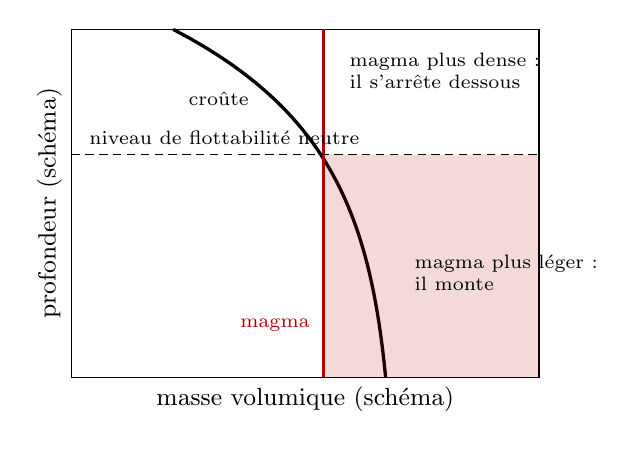
\begin{tikzpicture}[font=\scriptsize]
\begin{axis}[width=0.62\linewidth, height=6cm,
  xmin=0, xmax=1.15, ymin=0, ymax=1, y dir=reverse,
  xtick=\empty, ytick=\empty,
  xlabel={masse volumique (schéma)}, ylabel={profondeur (schéma)},
  label style={font=\small}, clip=false]
\addplot[very thick, black, domain=0:1, samples=40] ({0.25 + 0.55*(1 - exp(-3*x))}, {x});
\addplot[very thick, red!70!black] coordinates {(0.62,0) (0.62,1)};
\fill[red!70!black, opacity=0.15] (axis cs:0.62,0.36) rectangle (axis cs:1.15,1);
\draw[densely dashed] (axis cs:0,0.36) -- (axis cs:1.15,0.36);
\node[anchor=south west] at (axis cs:0.02,0.36) {niveau de flottabilité neutre};
\node[anchor=east, black] at (axis cs:0.46,0.20) {croûte};
\node[anchor=east, red!70!black] at (axis cs:0.61,0.85) {magma};
\node[anchor=west, align=left] at (axis cs:0.82,0.70) {magma plus léger~:\\il monte};
\node[anchor=west, align=left] at (axis cs:0.66,0.12) {magma plus dense~:\\il s'arrête dessous};
\end{axis}
\end{tikzpicture}
\par\smallskip{\small Le \omterm{def:b2:magma-emplacement:ascent}{niveau de flottabilité neutre} (schéma). La masse volumique
de la croûte augmente avec la profondeur, par compaction des sédiments et par le passage à
des roches plus denses ; un \omterm{def:b2:magma-emplacement:magma}{magma} de masse volumique fixée monte tant qu'il est plus léger que son
environnement (grisé) et s'étale là où les deux masses volumiques se rejoignent.}
\end{omfigure}

Un \omterm{def:b2:magma-emplacement:bodies}{pluton} doit se faire de la place. Il peut soulever son toit, comme le fait une \omterm{def:b2:magma-emplacement:bodies}{laccolite}~;
il peut écarter ses parois là où elles sont molles ; il peut remplir un espace ouvert par
une faille ; et il peut arracher son toit, bloc par bloc. Les grands \omterm{def:b2:magma-emplacement:bodies}{plutons} ont longtemps été
imaginés comme d'énormes réservoirs de \omterm{def:b2:magma-emplacement:magma}{magma} mis en place d'un seul coup. La datation a changé
cette image. Les zircons de la suite intrusive de Tuolumne, un \omterm{def:b2:magma-emplacement:bodies}{batholite} granitique en
Californie, montrent qu'elle a été mise en place entre \num{95} et \qty{85}{Ma}, les plus anciens
en bordure et les plus jeunes au centre, et l'une de ses unités seule sur plus
de \qty{3}{Ma}, entre \qty{92.8}{Ma} et \qty{88.8}{Ma}. Un seul corps de
\omterm{def:b2:magma-emplacement:magma}{magma} de \qty{5}{km} d'épaisseur et de \qty{20}{km} de large, mis en place à \qty{15}{km} de profondeur, aurait
refroidi sous \qty{750}{\celsius}, température à laquelle il est cristallisé à moitié, en
environ \num{500000}~ans. De tels \omterm{def:b2:magma-emplacement:bodies}{plutons} ont dû être édifiés par étapes
à partir de nombreuses intrusions plus petites, comme des nappes et des \omterm{def:b2:magma-emplacement:bodies}{dykes}, sur des millions d'années
(voir l'\cref{exo:b2:magma-emplacement:11}).
% ledger: glazner04:tuolumne

\begin{omfigure}
\centering
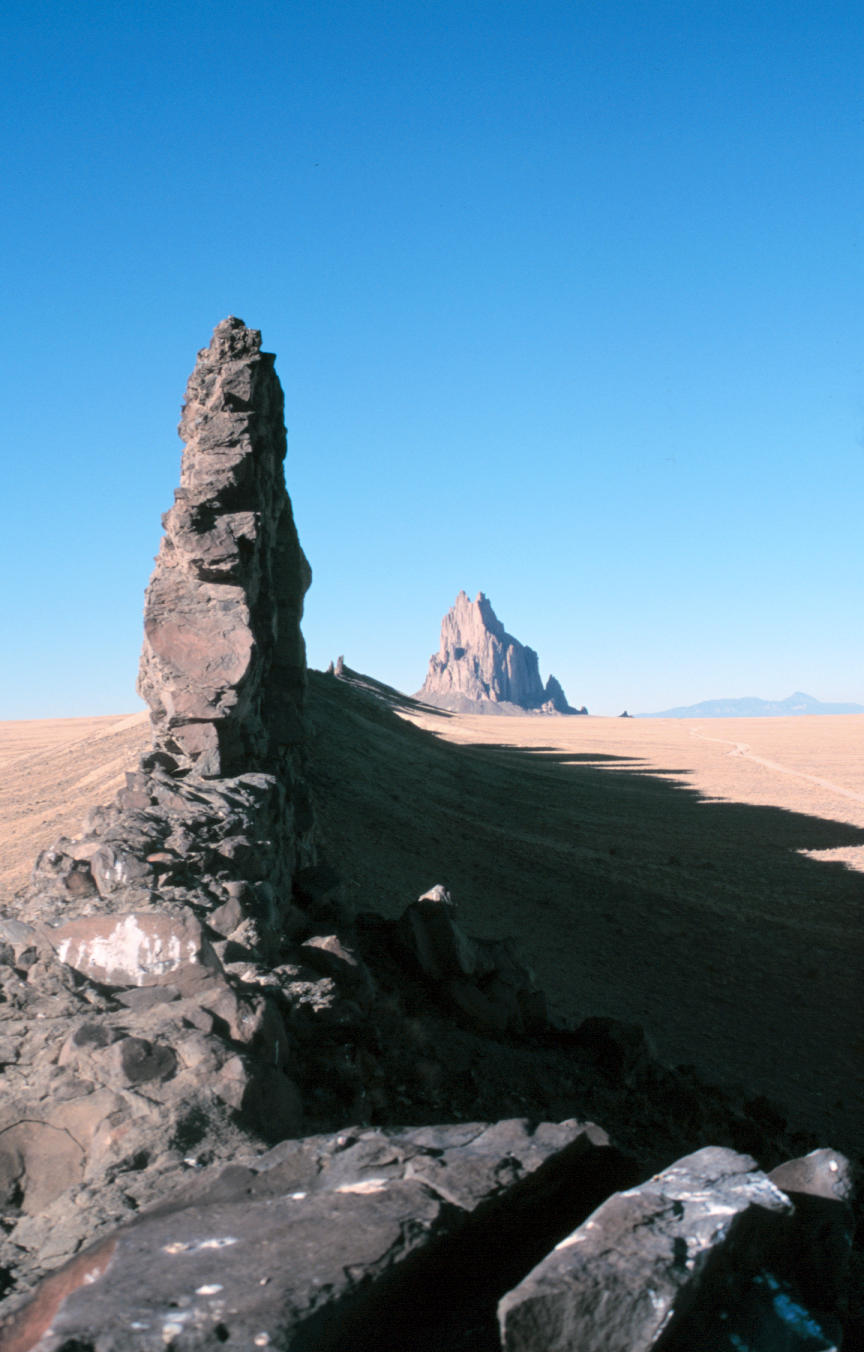
\includegraphics[width=0.3\linewidth]{images/book4/b2-shiprock-dyke.jpg}
\par\smallskip{\small Un \omterm{def:b2:magma-emplacement:bodies}{dyke} près de Shiprock, dans le Navajo Volcanic Field
(Nouveau-Mexique)~: la roche du \omterm{def:b2:magma-emplacement:bodies}{dyke} a mieux résisté à l'érosion que le grès et le schiste
qu'il recoupait, et se dresse aujourd'hui en muraille~; au loin, le culot volcanique d'où
rayonnent plusieurs \omterm{def:b2:magma-emplacement:bodies}{dykes} semblables. Photographie~: Dexter Perkins (CC0).}
\end{omfigure}

\section{Refroidissement et métamorphisme de contact}

Une intrusion perd sa chaleur par conduction vers les roches encaissantes. Le modèle le plus simple
traite l'intrusion et son encaissant comme un milieu conducteur unique de diffusivité
uniforme $\kappa$ : à l'instant zéro, une nappe d'épaisseur $b$ est à la température d'intrusion
$T_m$ et l'encaissant à $T_0$. La solution de l'équation de la chaleur, avec
$x$ compté depuis le milieu de la nappe, est
\[
T(x,t) = T_0 + \frac{T_m - T_0}{2}\left[\operatorname{erf}\frac{b/2 - x}{2\sqrt{\kappa t}}
+ \operatorname{erf}\frac{b/2 + x}{2\sqrt{\kappa t}}\right].
\]
La figure ci-dessous la représente pour un \omterm{def:b2:magma-emplacement:bodies}{sill} d'épaisseur \qty{100}{m}.
% ledger: delaney86b4:properties

\begin{proposition}[Température de contact]\label{prop:b2:magma-emplacement:contact}
Dans ce modèle, tant que $\sqrt{\kappa t}$ est petit devant $b$, la
température au contact de l'intrusion reste égale à la moyenne $(T_m + T_0)/2$ des
températures de l'intrusion et de l'encaissant.
\end{proposition}

\begin{proof}
Au contact, $x = b/2$, la première fonction d'erreur vaut $\operatorname{erf}0 = 0$ et
la seconde vaut $\operatorname{erf}(b/(2\sqrt{\kappa t}))$, proche de $1$ tant que
$b \gg 2\sqrt{\kappa t}$. Alors $T = T_0 + (T_m - T_0)/2$.
\end{proof}

Un \omterm{def:b2:magma-emplacement:bodies}{dyke} basaltique à \qty{1150}{\celsius} dans des roches à \qty{50}{\celsius} porte donc son contact à
\qty{600}{\celsius}. La chaleur de cristallisation, typiquement
\qtyrange{700}{1000}{MJ/m^3}, maintient le \omterm{def:b2:magma-emplacement:magma}{magma} chaud plus longtemps et élève cette valeur~:
avec \qty{900}{MJ/m^3} libérés entre \num{1150} et \qty{950}{\celsius}, le même
modèle donne \qty{690}{\celsius}, tandis que des conductivités dépendant de la température et des
roches encaissantes humides abaissent les deux estimations de 50 à \qty{75}{\celsius}.
% ledger: delaney86b4:dike, delaney86b4:properties

\begin{omfigure}
\centering
\begin{tikzpicture}
\begin{axis}[omrecord, width=0.86\linewidth, height=6cm,
  xmin=-200, xmax=200, ymin=0, ymax=1200,
  xlabel={distance au milieu du sill (\unit{m})},
  ylabel={température (\unit{\celsius})},
  legend pos=north east, legend style={font=\scriptsize},
  tick label style={font=\scriptsize}, label style={font=\small}]
\fill[gray!15] (axis cs:-50,0) rectangle (axis cs:50,1200);
\addplot[very thick, red!80!black] table[x=x_m, y=t1] {figdata/out/bachelor-2-magma-sill.dat};
\addlegendentry{1 an}
\addplot[very thick, orange!90!black] table[x=x_m, y=t2] {figdata/out/bachelor-2-magma-sill.dat};
\addlegendentry{10 ans}
\addplot[very thick, blue!60!black] table[x=x_m, y=t3] {figdata/out/bachelor-2-magma-sill.dat};
\addlegendentry{50 ans}
\addplot[very thick, black] table[x=x_m, y=t4] {figdata/out/bachelor-2-magma-sill.dat};
\addlegendentry{200 ans}
\draw[densely dashed, gray] (axis cs:-200,625) -- (axis cs:200,625);
\node[font=\scriptsize, gray!40!black, anchor=south west] at (axis cs:-198,625) {$(T_m + T_0)/2$};
\node[font=\scriptsize, anchor=south] at (axis cs:0,20) {sill};
\end{axis}
\end{tikzpicture}
\par\smallskip{\small Refroidissement conductif d'un \omterm{def:b2:magma-emplacement:bodies}{sill} de \qty{100}{m} d'épaisseur (grisé),
mis en place à \qty{1150}{\celsius} dans une roche à \qty{100}{\celsius}, avec
$\kappa = \qty{0.7e-6}{m^2/s}$ et sans chaleur latente. Le contact reste voisin de
\qty{625}{\celsius} pendant des décennies, tandis que la chaleur se diffuse dans l'encaissant ; après deux
siècles, le \omterm{def:b2:magma-emplacement:bodies}{sill} et son environnement forment une large zone chaude.}
\end{omfigure}
% ledger: delaney86b4:properties

L'échelle de temps du refroidissement est le temps que met la chaleur à diffuser à travers
l'intrusion, de l'ordre de $(b/2)^2/\kappa$ : environ \num{16} jours pour un \omterm{def:b2:magma-emplacement:bodies}{dyke}
de \qty{2}{m} de large, un siècle pour un \omterm{def:b2:magma-emplacement:bodies}{sill} de \qty{100}{m} d'épaisseur, cent mille ans
pour un \omterm{def:b2:magma-emplacement:bodies}{pluton} de quelques kilomètres. La chaleur latente l'allonge, et il en est de même
de la nécessité de solidifier le \omterm{def:b2:magma-emplacement:magma}{magma} plutôt que de simplement le refroidir.

\begin{proposition}[Solidification d'une intrusion]\label{prop:b2:magma-emplacement:stefan}
Soit du \omterm{def:b2:magma-emplacement:magma}{magma} à sa température de solidification $T_m$, de chaleur latente $L$ par unité
de volume, remplissant l'espace $y > 0$ à côté d'une roche encaissante à $T_0$ occupant $y < 0$, toutes deux
de capacité thermique $\rho c$ par unité de volume et de diffusivité $\kappa$. Le
front de solidification avance selon $y_s = 2\lambda\sqrt{\kappa t}$, où $\lambda$
est la racine de
\[
\frac{L\sqrt\pi}{\rho c\,(T_m - T_0)} = \frac{e^{-\lambda^2}}{\lambda\,(1 + \operatorname{erf}\lambda)},
\]
et le contact reste à $T_0 + (T_m - T_0)/(1 + \operatorname{erf}\lambda)$. Un \omterm{def:b2:magma-emplacement:bodies}{sill}
d'épaisseur $b$, qui se solidifie à partir de ses deux parois, est solide après
$t = b^2/(16\lambda^2\kappa)$.
\end{proposition}

\begin{proof}
Le \omterm{def:b2:magma-emplacement:magma}{magma} en avant du front reste à $T_m$, si bien que la chaleur ne circule que dans le solide
et dans l'encaissant, où l'on essaie $T = T_0 + (T_m - T_0)(1 + \operatorname{erf}\xi)/(1 +
\operatorname{erf}\lambda)$ avec $\xi = y/(2\sqrt{\kappa t})$. Toute fonction de $\xi$
de la forme $\alpha + \beta\operatorname{erf}\xi$ est solution de l'équation de la chaleur ; celle-ci
tend vers $T_0$ loin dans l'encaissant ($\xi \to -\infty$) et vaut $T_m$ sur le front
$\xi = \lambda$. En $y = 0$, elle donne la température de contact énoncée. Sur le front,
la chaleur latente libérée par le solide qui progresse, $L\,dy_s/dt = L\lambda\sqrt{\kappa/t}$
par unité d'aire et de temps, doit être évacuée par conduction, $k\,\partial T/\partial y = k(T_m -
T_0)\,e^{-\lambda^2}/[(1 + \operatorname{erf}\lambda)\sqrt{\pi\kappa t}]$. En égalant les
deux et en utilisant $k = \rho c\kappa$, on obtient l'équation de $\lambda$. Chaque paroi du
\omterm{def:b2:magma-emplacement:bodies}{sill} fait avancer son propre front, indépendamment tant que le cœur reste à $T_m$ ; les deux
fronts se rejoignent lorsque $2\lambda\sqrt{\kappa t} = b/2$.
\end{proof}

Avec la chaleur latente d'un basalte et un encaissant à environ \qty{100}{\celsius},
$\lambda$ vaut environ $0.65$~: un \omterm{def:b2:magma-emplacement:bodies}{sill} d'épaisseur \qty{100}{m} se solidifie en environ
soixante-dix ans, et son contact reste voisin de \qty{740}{\celsius} au lieu de
\qty{625}{\celsius} pendant ce temps. Le problème du week-end traite ce cas.
Comme le temps croît comme le carré de l'épaisseur, un \omterm{def:b2:magma-emplacement:bodies}{sill} dix fois plus épais
met cent fois plus de temps.

\begin{definition}[Auréole de contact et roches qui la composent]\label{def:b2:magma-emplacement:aureole}
Une \emph{bordure figée}\index{bordure figée} est la bordure à grain fin ou vitreuse d'une
intrusion, là où le \omterm{def:b2:magma-emplacement:magma}{magma} s'est refroidi vite contre une roche encaissante plus froide. Une
\emph{auréole de contact}\index{auréole de contact} est la zone de roche encaissante autour d'une
intrusion qui a été métamorphisée par sa chaleur. La \emph{cornéenne}\index{cornéenne} est la
roche dure, à grain fin et non foliée, que deviennent les argilites et les roches volcaniques dans une
auréole de contact. Le \emph{skarn}\index{skarn} est la roche formée là où des fluides magmatiques chauds
réagissent avec la roche encaissante carbonatée, en déposant des silicates de calcium--fer--magnésium
tels que grenat et pyroxène, souvent avec de la magnétite et des sulfures métalliques.
\end{definition}
% ledger: earle:intrusive-bodies, earle:skarn

Les \omterm{def:b2:magma-emplacement:aureole}{auréoles de contact} vont de quelques centimètres autour de petits \omterm{def:b2:magma-emplacement:bodies}{dykes} et \omterm{def:b2:magma-emplacement:bodies}{sills} à
plusieurs dizaines de mètres autour d'un grand stock, et le métamorphisme de contact couvre
environ \qty{300}{\celsius} à plus de \qty{800}{\celsius}. Une argilite devient une
\omterm{def:b2:magma-emplacement:aureole}{cornéenne}, un calcaire un marbre, un grès un quartzite. Un \omterm{def:b2:magma-emplacement:magma}{magma} mis en place en profondeur
dans des roches déjà chaudes ne produit presque aucune auréole : la largeur dépend de la
taille et de la température de l'intrusion ainsi que de la température de son encaissant, comme
le prévoit le modèle de refroidissement (voir l'\cref{exo:b2:magma-emplacement:12}). Les minéraux qui croissent dans une auréole,
et ce qu'ils disent de la température, appartiennent au \cref{ch:b2:metamorphic-facies} ;
les métaux que concentrent les \omterm{def:b2:magma-emplacement:aureole}{skarns} sont traités au \cref{ch:b2:ore-deposits}.
% ledger: earle:skarn

\begin{inthefield}[Lire les contacts d'un dyke]
\begin{minipage}[t]{0.6\linewidth}\vspace{0pt}
Lorsqu'un \omterm{def:b2:magma-emplacement:bodies}{dyke} affleure, un géologue suit d'abord ses contacts avec la roche
encaissante. Une bordure à grain plus fin ou plus vitreux que le centre du \omterm{def:b2:magma-emplacement:bodies}{dyke} indique
que le \omterm{def:b2:magma-emplacement:magma}{magma} a été refroidi contre une roche froide ; un \omterm{def:b2:magma-emplacement:bodies}{dyke} large de \qty{25}{cm}, étudié
sur la côte de Colombie-Britannique, présente des \omterm{def:b2:magma-emplacement:aureole}{bordures figées} de \qty{2}{cm} d'épaisseur. La roche
encaissante est examinée au contact pour y repérer une cuisson : un changement de couleur, un durcissement,
de nouveaux minéraux qui s'estompent à mesure qu'on s'éloigne du \omterm{def:b2:magma-emplacement:bodies}{dyke}. La largeur de la zone cuite et de
la \omterm{def:b2:magma-emplacement:aureole}{bordure figée}, rapportée à la largeur du \omterm{def:b2:magma-emplacement:bodies}{dyke}, indique à quelle température
se trouvait l'encaissant à l'arrivée du \omterm{def:b2:magma-emplacement:bodies}{dyke} ; un \omterm{def:b2:magma-emplacement:bodies}{dyke} sans \omterm{def:b2:magma-emplacement:aureole}{bordure figée} ni
auréole s'est mis en place dans des roches déjà chaudes. Des échantillons sont prélevés en travers
du \omterm{def:b2:magma-emplacement:bodies}{dyke}, de la bordure au centre, pour la géochimie de son liquide et pour la
taille de ses cristaux.
\end{minipage}\hfill
\begin{minipage}[t]{0.36\linewidth}\vspace{0pt}
\centering
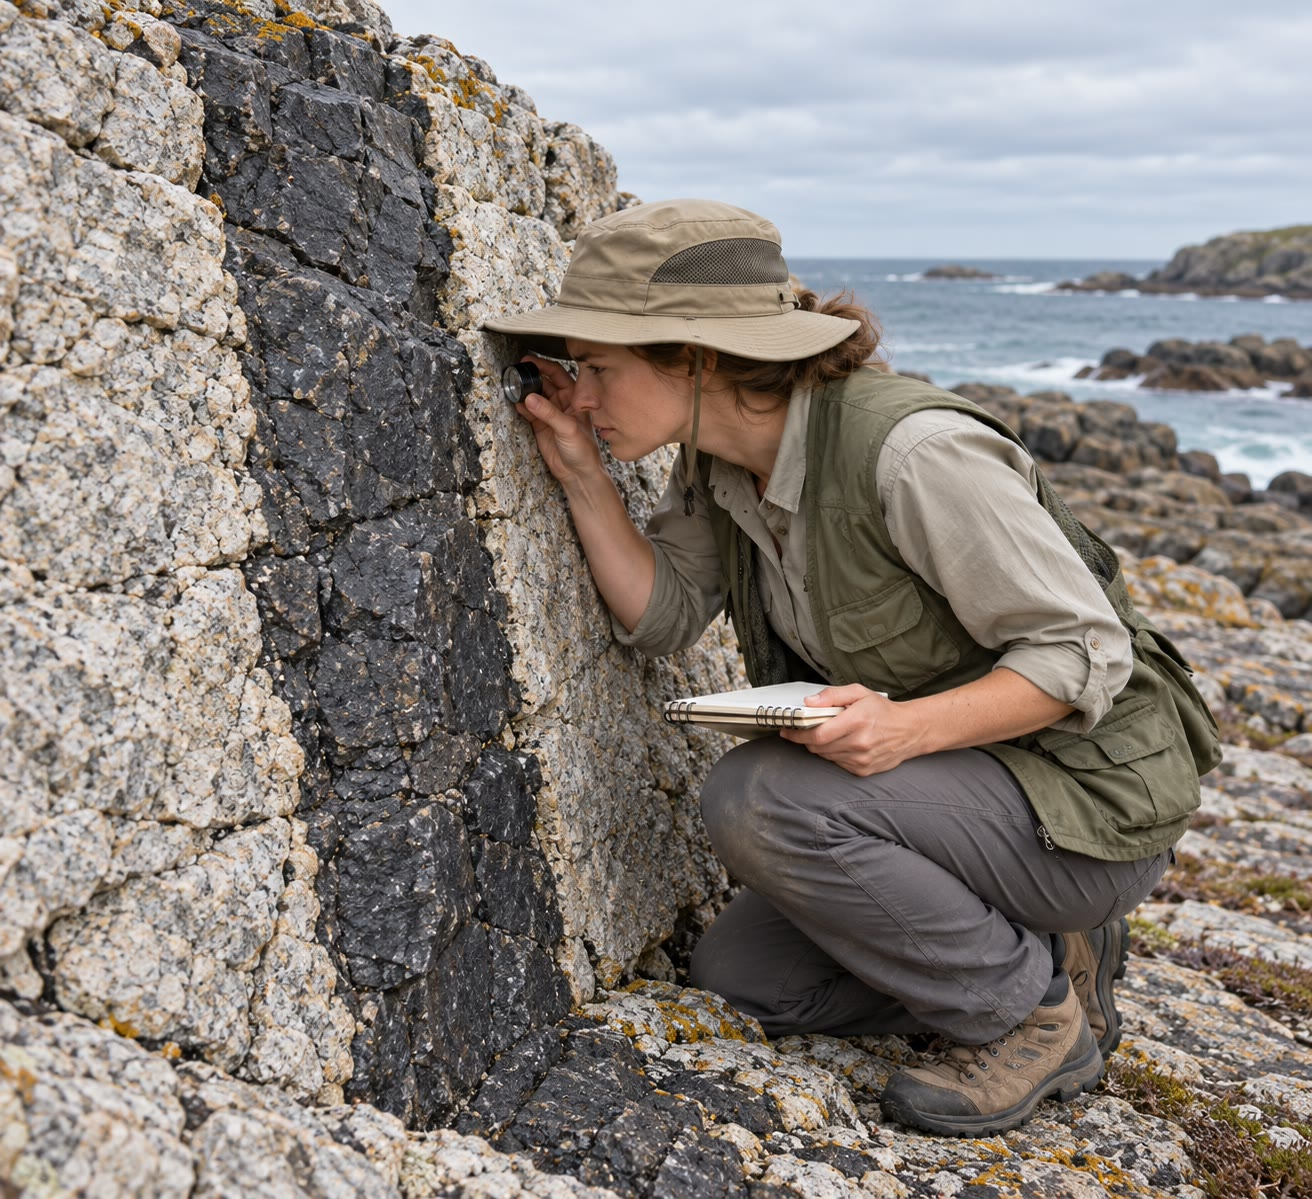
\includegraphics[width=\linewidth]{images/book4/ai/b2-dyke-contact.jpg}
\par\smallskip{\scriptsize Un géologue examinant le contact d'un \omterm{def:b2:magma-emplacement:bodies}{dyke} sombre avec
une roche encaissante claire (Illustration générée par IA.)}
\end{minipage}
\end{inthefield}
% ledger: earle:intrusive-bodies

\section{Exercices}

\begin{exercise}[$\star$]\label{exo:b2:magma-emplacement:1}
Pour les liquides granitiques hydratés, une équation ajustée sur des mesures donne
$\log_{10}\eta = [-3.545 + 0.833\ln w] + [9601 - 2368\ln w]/\{T - [195.7 + 32.25\ln
w]\}$, avec $\eta$ en \unit{Pa.s}, $w$ la teneur en eau en pour cent massique et $T$
en kelvins. Calculer $\log_{10}\eta$ à \qty{800}{\celsius} pour $w = 1$ et $w = 4$,
et le facteur par lequel les trois pour cent d'eau supplémentaires réduisent la viscosité.
\end{exercise}
% ledger: hd96:model

\begin{exercise}[$\star$]\label{exo:b2:magma-emplacement:2}
Avec la loi en racine carrée, $s = 0.44$ pour une rhyolite et $s = 0.34$ pour un basalte
(pour cent en masse par $\sqrt{\unit{MPa}}$), calculer la pression de saturation d'une
rhyolite à \qty{6}{\percent} d'eau et d'un basalte à \qty{0.5}{\percent}, ainsi que les
profondeurs correspondantes dans une croûte de masse volumique \qty{2600}{kg/m^3}
($g = \qty{9.81}{m/s^2}$).
\end{exercise}

\begin{exercise}[$\star$]\label{exo:b2:magma-emplacement:3}
Calculer la température de contact d'un \omterm{def:b2:magma-emplacement:bodies}{dyke} basaltique à \qty{1150}{\celsius}
mis en place dans des roches à \qty{50}{\celsius}, puis dans des roches à
\qty{400}{\celsius}. Lequel des deux \omterm{def:b2:magma-emplacement:bodies}{dykes} aura la \omterm{def:b2:magma-emplacement:aureole}{bordure figée} la plus large~?
\end{exercise}

\begin{exercise}[$\star$]\label{exo:b2:magma-emplacement:4}
Nommer chaque corps. (a) Une nappe de dolérite de \qty{30}{m} d'épaisseur placée entre deux couches
de grès sur \qty{20}{km}. (b) Une nappe verticale de basalte large de \qty{2}{m}
recoupant des calcaires horizontaux. (c) Un granite affleurant sur \qty{2000}{km^2},
formé d'une douzaine d'unités d'âges différents. (d) Une lentille de porphyre large de \qty{1}{km},
plane à sa base, au-dessus de laquelle les couches sont arquées vers le haut. (e) Une nappe horizontale
de basalte dans un granite.
\end{exercise}

\begin{exercise}[$\star\star$]\label{exo:b2:magma-emplacement:5}
Un liquide basaltique a $\eta_{\ell} = \qty{100}{Pa.s}$. Avec la relation d'Einstein--Roscoe
($R = 1.35$), calculer la viscosité du \omterm{def:b2:magma-emplacement:magma}{magma} contenant
\qty{5}{\percent}, \qty{20}{\percent}, \qty{40}{\percent} et \qty{60}{\percent} de
cristaux, et comparer la première avec la formule diluée d'Einstein. À quelle fraction
de cristaux la relation prévoit-elle le blocage~?
\end{exercise}

\begin{exercise}[$\star\star$]\label{exo:b2:magma-emplacement:6}
Un \omterm{def:b2:magma-emplacement:magma}{magma} de masse volumique inférieure de \qty{300}{kg/m^3} à celle de ses parois monte dans un \omterm{def:b2:magma-emplacement:bodies}{dyke}.
(a) Pour un basalte ($\eta = \qty{100}{Pa.s}$, $\rho = \qty{2700}{kg/m^3}$) dans un \omterm{def:b2:magma-emplacement:bodies}{dyke}
large de \qty{1}{m}, calculer la vitesse moyenne, le débit par mètre de \omterm{def:b2:magma-emplacement:bodies}{dyke}, le
nombre de Reynolds et le temps pour monter \qty{10}{km}. (b) Même calcul de temps pour une rhyolite de
\qty{e6}{Pa.s} dans un \omterm{def:b2:magma-emplacement:bodies}{dyke} large de \qty{1}{m}, puis de \qty{10}{m}. (c) Un \omterm{def:b2:magma-emplacement:bodies}{dyke}
large de \qty{1}{m} perd sa chaleur en un temps de l'ordre de $(w/2)^2/\kappa$, avec $\kappa =
\qty{1e-6}{m^2/s}$~: laquelle des trois remontées peut réussir~?
\end{exercise}

\begin{exercise}[$\star\star$]\label{exo:b2:magma-emplacement:7}
Un \omterm{def:b2:magma-emplacement:magma}{magma} de masse volumique \qty{2400}{kg/m^3} à \qty{900}{\celsius} libère
\qty{1}{\percent} de sa masse en vapeur d'eau. En assimilant la vapeur à un gaz parfait
($R = \qty{8.314}{J/(mol.K)}$, \qty{18.015}{g/mol}), calculer la fraction volumique de
gaz dans le \omterm{def:b2:magma-emplacement:magma}{magma} à \qty{100}{MPa}, \qty{10}{MPa} et \qty{0.1}{MPa}. Laquelle des
trois valeurs est la moins fiable, et pourquoi~?
\end{exercise}

\begin{exercise}[$\star\star$]\label{exo:b2:magma-emplacement:8}
Dans un bassin, la masse volumique des roches croît avec la profondeur $z$ selon $\rho(z) =
2300 + 60\,z$ (\unit{kg/m^3}, $z$ en \unit{km}) jusqu'à \qty{10}{km}. (a) Où se trouve
le \omterm{def:b2:magma-emplacement:ascent}{niveau de flottabilité neutre} d'un liquide basaltique de \qty{2650}{kg/m^3}~? (b) Le
modèle de masse volumique de ce chapitre montre qu'un pour cent d'eau dissoute abaisse
la masse volumique d'un liquide basaltique d'environ \qty{70}{kg/m^3}. Où s'arrête un liquide
contenant un pour cent d'eau de plus~? (c) Quelle est la force de flottabilité par mètre cube
du liquide sec situé \qty{2}{km} sous son \omterm{def:b2:magma-emplacement:ascent}{niveau de flottabilité neutre}~?
\end{exercise}

\begin{exercise}[$\star\star$]\label{exo:b2:magma-emplacement:9}
Supposons un \omterm{def:b2:magma-emplacement:ascent}{diapir} granitique de rayon \qty{1}{km} et de déficit de masse volumique
\qty{300}{kg/m^3} qui monte à travers une croûte inférieure de viscosité \qty{e19}{Pa.s}. Calculer
sa vitesse de Stokes (sphère rigide) en millimètres par an et le temps pour monter
\qty{10}{km}. Comparer avec l'échelle de temps $a^2/\kappa$ de son refroidissement, avec $\kappa
= \qty{1e-6}{m^2/s}$. Que conclure~?
\end{exercise}

\begin{exercise}[$\star\star\star$]\label{exo:b2:magma-emplacement:10}
L'eau se dissout dans un liquide à la fois sous forme de molécules, $x_m = K_1 f$, et sous forme de
groupes hydroxyles, $x_{\mathrm{OH}}^2 = K_2 x_m$ (l'oxygène du liquide étant en large excès), de sorte que
l'eau dissoute totale vaut $x = x_m + x_{\mathrm{OH}}/2$. (a) Exprimer $x$ en
fonction de $f$ et montrer qu'elle se comporte comme $\sqrt f$ à faible $f$ et comme $f$ à
fort $f$. (b) À quelle fugacité les deux formes d'eau sont-elles également abondantes~? (c)
Avec $K_1 = \qty{1e-4}{MPa^{-1}}$ et $K_2 = 0.2$, calculer cette fugacité, ainsi que la
part de l'eau dissoute sous forme d'hydroxyle à \qty{100}{MPa}.
\end{exercise}

\begin{exercise}[$\star\star\star$]\label{exo:b2:magma-emplacement:11}
Un \omterm{def:b2:magma-emplacement:bodies}{pluton} granitique de \qty{1000}{km^3} est édifié en \qty{4}{Ma}. (a) Calculer
son apport moyen de \omterm{def:b2:magma-emplacement:magma}{magma} en \unit{km^3} par an et en \unit{m^3} par seconde. (b) Un
seul \omterm{def:b2:magma-emplacement:bodies}{dyke} long de \qty{1}{km} et large de \qty{2}{m}, avec une vitesse moyenne de
\qty{0.8}{m/s}, l'alimente~: combien de temps ce \omterm{def:b2:magma-emplacement:bodies}{dyke} mettrait-il pour apporter tout le
\omterm{def:b2:magma-emplacement:bodies}{pluton}~? Quelle fraction des \qty{4}{Ma} cela représente-t-il~? (c) Si le \omterm{def:b2:magma-emplacement:bodies}{pluton} est formé de
nappes d'épaisseur \qty{20}{m} et de \qty{10}{km} sur \qty{10}{km}, combien de nappes
faut-il, et quel délai sépare en moyenne deux d'entre elles~? (d) Avec
$\lambda = 0.65$ et $\kappa = \qty{0.7e-6}{m^2/s}$, combien de temps une nappe met-elle pour
se solidifier~? Le \omterm{def:b2:magma-emplacement:bodies}{pluton} est-il jamais un seul grand corps de \omterm{def:b2:magma-emplacement:magma}{magma}~?
\end{exercise}

\begin{exercise}[$\star\star\star$]\label{exo:b2:magma-emplacement:12}
Loin d'un \omterm{def:b2:magma-emplacement:bodies}{dyke} mince de largeur $b$ (à des distances $x \gg b$), sa chaleur agit comme une
source plane instantanée : $T - T_0 = (T_m - T_0)\,b\,e^{-x^2/(4\kappa
t)}/\sqrt{4\pi\kappa t}$. (a) Montrer qu'à la distance $x$ la température est maximale à
$t^* = x^2/(2\kappa)$, et que cette élévation maximale vaut $\Delta T_{\max} = (T_m -
T_0)\,b/(x\sqrt{2\pi e})$. (b) Pour un \omterm{def:b2:magma-emplacement:bodies}{dyke} large de \qty{2}{m} avec $T_m - T_0 =
\qty{1100}{K}$, à quelle distance la roche se réchauffe-t-elle d'au plus \qty{100}{K}, et
quand ($\kappa = \qty{0.7e-6}{m^2/s}$)~? (c) Pourquoi les auréoles des \omterm{def:b2:magma-emplacement:bodies}{dykes} minces sont-elles si
étroites~?
\end{exercise}

\section{Problème~: le sill sous le plateau}

\begin{problem}[{Problème du week-end --- suivre un magma basaltique depuis son dyke d'alimentation
jusqu'à un sill, son eau et le temps que met le sill à se solidifier}]
\label{pb:b2:magma-emplacement:1}
Sous un plateau imaginaire, des sédiments (schiste et grès) de masse volumique moyenne
\qty{2450}{kg/m^3} reposent à \qty{3.0}{km} de profondeur sur un socle cristallin de
masse volumique \qty{2800}{kg/m^3}. Un \omterm{def:b2:magma-emplacement:magma}{magma} basaltique est monté depuis \qty{15}{km} par un \omterm{def:b2:magma-emplacement:bodies}{dyke}
large de \qty{2.0}{m} et s'est étalé à la base des sédiments en un \omterm{def:b2:magma-emplacement:bodies}{sill} de dolérite
d'épaisseur \qty{100}{m}. Données~: température d'intrusion \qty{1150}{\celsius} ; loi de viscosité du liquide
$\log_{10}\eta = -4.55 + 5510/(T - 611)$ ($T$ en kelvins) ; masse volumique du liquide
avec son eau \qty{2710}{kg/m^3} ; \qty{20}{\percent} de cristaux en volume
(Einstein--Roscoe, $R = 1.35$) ; eau dissoute \qty{0.40}{\percent}, solubilité
$s = 0.34$ pour cent par $\sqrt{\unit{MPa}}$ ; température de l'encaissant au niveau du \omterm{def:b2:magma-emplacement:bodies}{sill}
\qty{100}{\celsius} ; $\kappa = \qty{0.7e-6}{m^2/s}$, $\rho c = \qty{2.5}{MJ/(m^3.K)}$,
chaleur latente \qty{900}{MJ/m^3}, le \omterm{def:b2:magma-emplacement:magma}{magma} étant considéré comme se solidifiant à sa
température d'intrusion ; $g = \qty{9.81}{m/s^2}$ ; une année vaut \qty{3.156e7}{s}.

\medskip\noindent\textbf{Partie I --- Le magma.}
\begin{enumerate}
\item Calculer $\log_{10}\eta$ et $\eta$ du liquide à \qty{1150}{\celsius}
(\qty{1423}{K}).
\item Même question à \qty{1100}{\celsius}. De quel facteur la viscosité change-t-elle sur
ces \qty{50}{K}~?
\item Calculer la viscosité du \omterm{def:b2:magma-emplacement:magma}{magma} avec ses cristaux à
\qty{1150}{\celsius}.
\item À quelle fraction de cristaux la relation d'Einstein--Roscoe ferait-elle
bloquer le \omterm{def:b2:magma-emplacement:magma}{magma}~? Comparer avec l'estimation de terrain de la fin de l'écoulement d'ensemble.
\item Calculer la différence de masse volumique entre le \omterm{def:b2:magma-emplacement:magma}{magma} et le socle, et entre le \omterm{def:b2:magma-emplacement:magma}{magma} et
les sédiments.
\item Calculer la pression lithostatique au niveau du \omterm{def:b2:magma-emplacement:bodies}{sill}.
\end{enumerate}

\noindent\textbf{Partie II --- Remontée dans le dyke.}
\begin{enumerate}[resume]
\item Calculer le gradient de pression de flottabilité $\Delta\rho\,g$ qui entraîne le \omterm{def:b2:magma-emplacement:magma}{magma}
à travers le socle.
\item Calculer la vitesse moyenne du \omterm{def:b2:magma-emplacement:magma}{magma} dans le \omterm{def:b2:magma-emplacement:bodies}{dyke}.
\item Calculer le débit par mètre de \omterm{def:b2:magma-emplacement:bodies}{dyke}, et le débit total si le \omterm{def:b2:magma-emplacement:bodies}{dyke} est
long de \qty{1.0}{km}.
\item Calculer le nombre de Reynolds de l'écoulement. Est-il laminaire~?
\item Combien de temps le \omterm{def:b2:magma-emplacement:magma}{magma} met-il pour monter de \qty{15}{km} à \qty{3.0}{km}~?
\item Comparer avec l'échelle de temps $(w/2)^2/\kappa$ sur laquelle le \omterm{def:b2:magma-emplacement:bodies}{dyke} perd sa
chaleur. Peut-il rester ouvert~?
\item Expliquer pourquoi le \omterm{def:b2:magma-emplacement:magma}{magma} s'est arrêté à \qty{3.0}{km} et s'est étalé latéralement, en utilisant
le vocabulaire du chapitre.
\end{enumerate}

\noindent\textbf{Partie III --- L'eau.}
\begin{enumerate}[resume]
\item Calculer la pression de saturation de l'eau du liquide, et la profondeur, dans les
sédiments, où elle est atteinte.
\item Quelle quantité d'eau le liquide peut-il contenir au niveau du \omterm{def:b2:magma-emplacement:bodies}{sill}~? Le \omterm{def:b2:magma-emplacement:magma}{magma} du \omterm{def:b2:magma-emplacement:bodies}{sill}
exsolve-t-il de l'eau~?
\item Les vésicules de la \omterm{def:b2:magma-emplacement:aureole}{bordure figée} du \omterm{def:b2:magma-emplacement:bodies}{sill} contiennent surtout du CO$_2$. Expliquer.
\item Si la totalité des \qty{0.40}{\percent} d'eau sortait en surface, à
\qty{1150}{\celsius} et \qty{0.1}{MPa}, quelle fraction volumique du \omterm{def:b2:magma-emplacement:magma}{magma} occuperait
la vapeur (gaz parfait)~?
\end{enumerate}

\noindent\textbf{Partie IV --- Refroidissement et solidification.}
\begin{enumerate}[resume]
\item En négligeant la chaleur latente, calculer la température de contact du \omterm{def:b2:magma-emplacement:bodies}{sill}.
\item En négligeant la chaleur latente, calculer la température \qty{10}{m} au-dessus du
contact supérieur \num{10}~ans après l'intrusion.
\item Même modèle : calculer la température au milieu du \omterm{def:b2:magma-emplacement:bodies}{sill} après
\num{10}~ans et \num{50}~ans.
\item Même modèle : à \qty{80}{m} au-dessus du contact supérieur, calculer la température après
\num{300}, \num{363} et \num{420} ans. La roche atteint-elle jamais
\qty{300}{\celsius}~?
\item Calculer $L\sqrt\pi/(\rho c\,(T_m - T_0))$ pour le \omterm{def:b2:magma-emplacement:bodies}{sill}.
\item Évaluer $e^{-\lambda^2}/(\lambda(1 + \operatorname{erf}\lambda))$ pour $\lambda = 0.64$,
$0.65$ et $0.66$ ($\operatorname{erf}0.64 = 0.6346$, $\operatorname{erf}0.65 = 0.6420$,
$\operatorname{erf}0.66 = 0.6494$), et donner $\lambda$ à deux décimales.
\item En tenant compte de la chaleur latente, calculer la température de contact pendant que le \omterm{def:b2:magma-emplacement:bodies}{sill}
se solidifie. Pourquoi est-elle plus élevée qu'à la question~18~?
\item Calculer l'échelle de temps $(b/2)^2/\kappa$ en années.
\item Calculer le temps que met le \omterm{def:b2:magma-emplacement:bodies}{sill} à se solidifier, en années, le nombre clé de
ce problème, et expliquer pourquoi il est plus court que l'échelle de temps de la dernière
question, bien qu'il faille évacuer la chaleur latente.
\end{enumerate}
\end{problem}
% ledger: grd08:model, kolz22:einstein-roscoe, glazner04:tuolumne, moore98:h2o, lowenstern01:co2, delaney86b4:properties
